\subsection{POMDP}
We face a Partially Observed Markov Decision Process (POMDP), which we define as the tuple $(S,A,O,b_o,T,\Omega,R,\gamma,F)$, where:
\begin{itemize}
  \item $S$ is a set of discrete states, $A$ is a set of discrete actions, and $O$ is a set of continuous observations.
  \item $b_o$ is the initial belief state.
  \item $T(s,a,s') = P(s_{t+1} = s | a_t = a, s_t = s)$ is the distribution describing the probability of transitioning from state $s$ to state $s'$ upon taking action $a$.
  \item $\Omega(o,s,a) = P(o_{t+1}=o | a_t = a, s_{t+1} = s)$ is the distribution describing the probability of observing $o$ from state $s$ after taking action $a$.
  \item $R(s,a)$ is the reward signal received when executing action $a$ in state $s$.
  \item $F$ is the deadline to termination.
\end{itemize}
Our goal is to learn the optimal policy $\pi$, which is a mapping from belief states to actions.

\subsection{State representation}
For all approaches described later, the state $s \in S$ is fully defined by the time $T$, and the class of the bounding box centered at each location.
We augment the $K$ classes with a ``background'' class.
Note that each object in the image is assigned to exactly one location.
The number of states is exponential in $N$, which is on the order of $10000$ in our applications.\comment{$T (K+1)^N$ states.}
We are dealing with a static image and our actions do not change the underlying state, so $T(s,a,s') = \delta_{s, s'}$ where $\delta$ is the Kronecker delta function.

The belief state is supposed to be a distribution over ``physical'' states.
We model the belief state as a Conditional Random Field (CRF) over the $N$ locations in the image pyramid, where a node $y_{i} \in Y$ is an integer $0 \dots K$, according to the class whose bounding box we believe is centered at location $i$ (background is $0$).

For each node $y_i$, there are $\sum_{k=1}^K P_k$ nodes $z_{ikp}$, which represent a classifier's confidence in the corresponding $y_i$ node \note{(in some way)}.
Two nodes $y_i$ and $z_{ikp}$ are connected with weight $w_{kp}$.
This weight in a sense represents our confidence in the classifier $c_kp$.
We also leave open the possibility of extra nodes $z_{ikp'}$ to model contextual cues or \emph{a priori} beliefs.

The connections between two nodes $y_i$ and $y_j$ are defined by the spatial context feature $d_{ij}$ (represented in~\autoref{fig:dij}) and the weights $w_{y_i,y_j}$, which encode valid geometric configurations of object classes $y_i$ and $y_j$.
\begin{figure}[h!]
  \caption{Figure from~\cite{Desai2009}.}
  \centering
    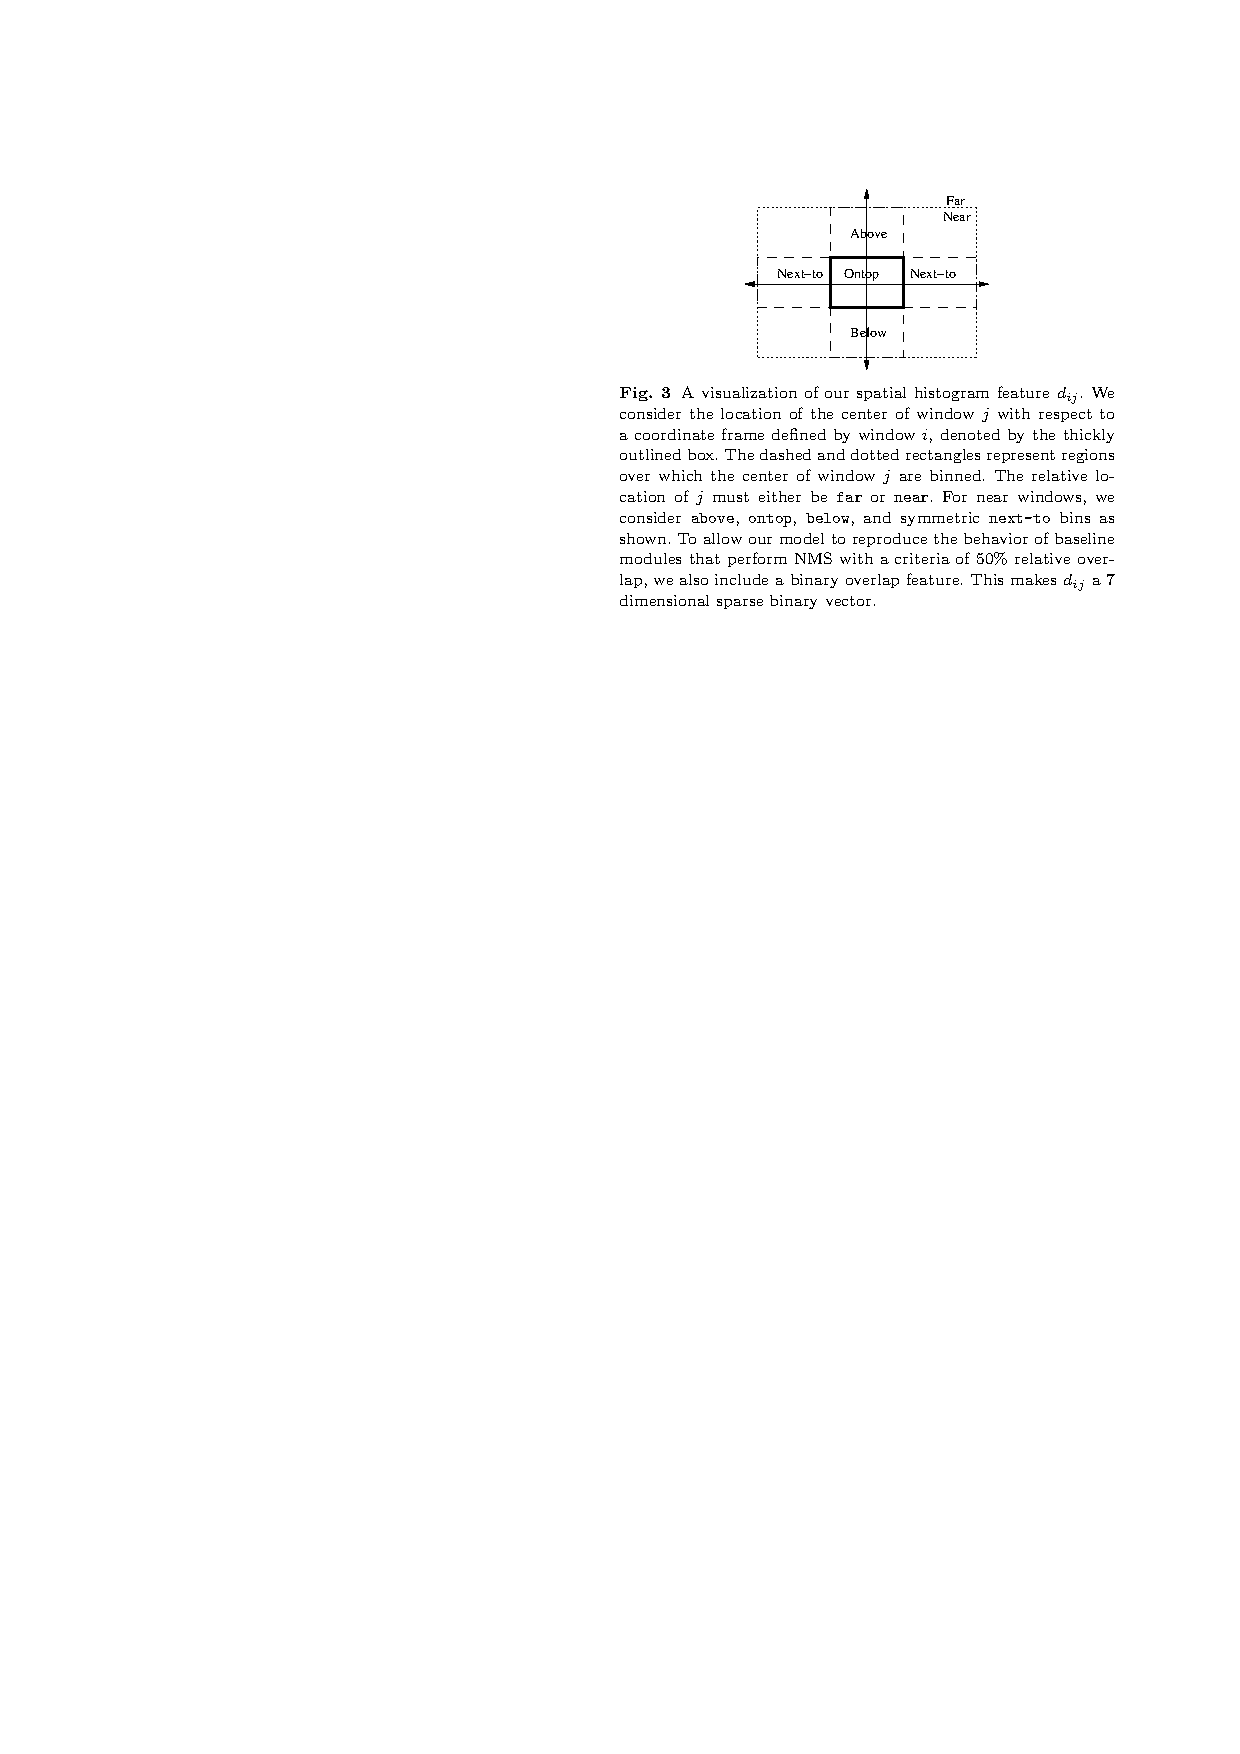
\includegraphics[width=0.7\textwidth]{../figures/dij.pdf}
  \label{fig:dij}
\end{figure}

This way of modeling the underlying state of the image is similar to the one used in~\cite{Desai2009}.
In fact, we rely on their method of greedy forward search to do inference in the CRF and learn the parameters; inference of the physical state from our belief state is described in~\autoref{sec:rewards}.

\subsection{Actions and Observations} \label{sec:actions}
Actions are defined by a choice of location $i$ and partial detector $c_{kp}$, making for $N \sum_{k=1}^K P_k$ possibilities.

Upon executing an action, the observation $o$ we get back is the decision of the classifier (or its score, if provided).
The observation updates the corresponding node $z_{ikp}$.
We can propagate this update through the CRF with an iteration of belief propagation, or alternatively, we can fully ``resolve'' our CRF by running a greedy forward search (details in~\autoref{sec:rewards}).
We can do this at every action, every fixed number of actions, or upon taking a special action.

We may also want to think of executing actions in batches, such as ``evaluate $c_{kp}$ at all locations,'' or ``evaluate all $c$ at a location $i$.''
We can represent such sets of actions as a special action.

\subsection{Deadline} \label{sec:deadlines}
We express $F$ in units of expected time per action, such that taking action $a$ with time cost $\tau$ advances $T$ by $\tau$.
We determine $\tau$ by averaging the wall clock time of executing $a$; this is done for all $a$ prior to running the POMDP learner.

Toward our goal is Anytime performance starting at some fixed deadline $F$ (see~\autoref{sec:evaluation}), our training procedure enforces the deadline stochastically, terminating the agent at any random $T \geq F$.

\subsection{Outputting Detections and Rewards} \label{sec:rewards}
$Y$ in our belief state represents the detections, and $Z$ provides confidences for $Y$.

Recall that we cannot have detections of two different classes at the same location, and that the PASCAL evaluation will penalize all but one detections of the same class at overlapping locations.
For this reason, most detection systems that ``assign content to locations'' run a post-processing non-maximum suppression step~\cite{Felzenszwalb2010a}.
In a multi-class setting, it is better to resolve such ambiguities with a principled system to model both inter- and intra-class, and short- and long-range interactions.

Our belief state is modeled after such a system, and we simply run a greedy forward search to maximize the energy of our CRF to pick our final detections~\cite{Desai2009}.
The energy of the CRF is given as
\begin{equation}
  S(Y,Z) = \sum_{i,j} w_{y_i,y_j}^T d_{ij} + \sum_{i,kp} w_{kp} z_{ikp}
\end{equation}
In brief, the greedy search starts out with an empty set of detections, and proceeds to pick those $y_i$ that maximize $\Delta S(Y,Z)$.
It was shown to be optimal for nearly all images ($\approx98\%$) in the PASCAL set (and compared against Loopy BP and Tree-ReWeighted BP)~\cite{Desai2009}.

The theoretical explanation for this comes from the work on \emph{submodular functions}.
The rough idea is that to maximize functions where adding an element to a large set has less effect than adding an element to a small set, greedy algorithms often have theoretical guarantees of near-optimal performance.
The more pairwise connections are non-positive in the CRF, the more submodular it is.
\note{Mention percentage of our learned connections that are non-positive to justify this.}

After every action, $R(s,a)$ is assigned according to the AP of these detections.
The program is terminated at time $F$.

\subsection{Some Example Policies}
To get a feel for how different detection strategies fit into our framework, we go through some examples, in order of increasing complexity.

\paragraph{Sliding window}
Here, we take actions that run whole detectors and not their individual classifiers.
We featurize the belief state with just two things: the location $i$ and class $k$ of the last action.
The policy simply increments these in order, cycling through either locations or classes.

\paragraph{Sliding window, cascaded}
Now we pick the actual classifier, not just the detector, so let's store $i$ and $c_{kp}$ of the last action.
The policy can use the thresholds that the Cascaded DPM detector learned: if observation $o$ is past threshold for $c_{kp}$, then the next action will be $c_{k{p+1}}$ at the same location; otherwise, we move on to another location or class.

\paragraph{Saliency-driven}
Once again we take actions that run whole detectors.
Our policy first computes a simple saliency map for the image (for example, as in~\cite{Alexe2010}).
The belief state is featurized by the location of the current unexamined (picked less than $K$ times) max in the saliency map and the class $k$ of the last action.
The policy is to simply sample locations in order of saliency, running all detectors at a location before proceeding to the next.

\paragraph{Class prior-driven}
On the training set, we compute $K$ canonical object likelihood maps.
We featurize the belief state with the current unexamined (picked less than $1$ time) max of each likelihood map.
Our policy is to run the detector for the class $k$ at the location $i$ with the largest likelihood among these maps.

\paragraph{Root model score-driven, cascaded}
The first stage of the cascaded DPM detector is a PCA-reduced root filter.
Our policy has two stages.
First, it follows a modified \textbf{sliding window} policy to run the fast root filter everywhere in the image, for all classes.
Then, it follows a modification of the \textbf{Class prior-driven} policy, with the class priors given by the root filter scores, and classifier actions picked as in \textbf{Sliding window, cascaded}.

\paragraph{Coarse-to-fine, inspired by~\cite{Pedersoli2011}}
As above, except in between the stages, we resolve our belief state CRF (which basically does NMS in addition to other things).
This is similar to what they do in~\cite{Pedersoli2011}: run NMS after root filter scoring, then run higher-resolution parts and resolve them again, although we don't do the latter.

\paragraph{Coarse-to-fine, with smart featurization}
As explained in~\autoref{sec:discretization_and_featurization}, we can use low-resolution templates and the lower-scale part of the image pyramid to get estimates on the detections in the higher-scale part of the pyramid.

Our policy first computes only the lower scales of the feature pyramid, and otherwise follows the \textbf{Root model score-driven, cascaded} policy with a low-res root filter.
\aside{
\paragraph{Multi-scale models}As explained in~\autoref{sec:discretization_and_featurization}, it has been shown that one should not run high-resolution part-based models to look for small objects in the image pyramid~\cite{Park2010}.
Their approach learns when to use a low-resolution model and when to use a high-res model, and trains the combined model jointly.
Deciding when to use the low-res model could be part of a policy.
}